%!TEX root = main.tex

\section{Application to Super Resolution Deconvolution}
\label{sec:application}

    Deconvolution is a classical imaging inverse problem, appearing in various practical applications such as microscopy, photography or astronomy. It consists in recovering a high resolution image from blurred observations, possibly corrupted by various artifacts (measurement noise, external illumination, etc).
    The presence of background information in the signal to recover, even with a small intensity, significantly deteriorates the quality of traditional sparsity-based single-component reconstruction methods.

    In this section, we illustrate our representer theorem for a deconvolution composite optimization problem. We first emphasize the decoupling in the specific case of \emph{measures-plus-Hilbert} signal before performing actual reconstructions using a grid-based approximation of continuous-domain sparse signals.

    % In this section, we consider a composite signal model and illustrate the benefits of our representer theorem for a deconvolution optimization problem. In particular, composite modeling accurately recovers the unknown signal in situations where single-component problems fail to distinguish foreground from background information. Additionally, using a decoupled numerical procedure reduces the computation time compared to a direct 2-variables approach of the composite optimization problem.

    % The numerical experiments in this section have been implemented with the Python programming language based on the optimization package \texttt{Pyxu} \cite{pyxu-framework}. All the simulations have run on a workstation with 2 CPUs Intel Xeon E5-2680 v3 \@2.5 Ghz, 30 MB cache and 24 threads each. 
    \subsection{Definition of the composite model}
    \label{sec:comp:model}

        % We consider a composite deconvolution inverse problem in which the signal to recover is the sum of a sparse foreground component and a smooth background component.   
        % Such scenario is inspired from Single Molecule Localization Microscopy (SMLM) in which the signal of interest is an image of fluorescent molecules \cite{sage2019smlm}.
        % % The measurement procedure is modeled as a convolution with the point-spread function (PSF) of the microscope.
        % The action of the microscope on the scene is modeled by a convolution with its known point-spread function (PSF).
        % Out-of-focus particles appear more spread-out and fainter than the objects in the focal plan, hence motivating for a composite model with a sparse component to account for the foreground and a smooth one for the background.
        % Moreover, using a continuous signal model is relevant for SMLM as it is possible to reach a resolution below the diffraction limit, relying on the sparse nature of the observed molecules \cite{huang2017super,denoyelle2019sliding,laville2021sparse}.
        
        We consider a scenario inspired from Single Molecule Localization Microscopy (SMLM) in which the signal of interest is an image of fluorescent molecules \cite{sage2019smlm}. Out-of-focus particles appear more spread-out and fainter than the objects in the focal plan, hence motivating for a composite model. Moreover, using a continuous signal model is relevant for SMLM as it is possible to reach a resolution below the diffraction limit, relying on the sparse nature of the observed molecules \cite{huang2017super,denoyelle2019sliding,laville2021sparse}.


        % \subsubsection{Problem definition}
        We first describe a simplified composite inverse problems which mimics the characteristics of SMLM recovery. The measurements $\bm{y}\in\R^L$ are expressed as
        \begin{equation*}
            \bm{y} \approx S \left\{g * (s_1^\dagger + s_2^\dagger)\right\}.
        \end{equation*}
        in which the ground truth signal $s^\dagger := s_1^\dagger + s_2^\dagger$ is the sum of a sparse foreground component $s_1^\dagger \in \mathcal{B}$ and a smooth background component $s_2^\dagger \in \mathcal{H}$. The action of the microscope on the scene is modeled as the convolution with the \emph{point-spread function (PSF)} $g$, before sampling on the grid of observation pixels with the operator $S$.


        \subsubsection{Function spaces}
            For $d \in \mathbb{N}^*$, let $\mathcal{X} = \mathbb{R}^d$ be the continuous domain of the $d$-dimensional signal to recover $s^\dagger$. 

            We consider the classical model of Radon measures $\mathcal{B} = \mx$, in which sparse signals can be represented with Dirac impulses. The \textit{total-variation norm} $\norm{\cdot}_\mathcal{M}$ on $\mx$ is known to promote sparse solutions when used as a regularizer for optimization problems \cite{unser2017splines}. For $\czx$ the space of continuous vanishing functions on $\mathcal{X}$, which is the predual of $\mx$, we recall the dual definition of the total-variation norm
            \begin{equation*}
                \forall m \in \mx, \quad \lVert m \rVert_\mathcal{M} = \underset{\substack{\varphi \in \czx \\ \| \varphi \|_\infty = 1}}{\sup} \int_\mathcal{X} \varphi(x) \mathrm{d}m(x).
            \end{equation*}
            
            % For the smooth background component $s_2$, we consider the Hilbert space of square integrable functions $\mathcal{H} = \ldx$ equipped with the inner product
            % \begin{equation*}
            %     \forall f, h \in \ldx, \quad \langle f, h\rangle_2 = \int_\mathcal{X} f(x) h(x) \mathrm{d}x.
            % \end{equation*}
            % The resulting Hilbert norm over $\ldx$ is noted as $\norm{\cdot}_2$.

            For the smooth background component $s_2$, we consider the Hilbert space $\cH = \cHk$ the RKHS\footnote{\textit{Reproducing Kernel Hilbert Space}.} induced by the Gaussian kernel $k: \cX \times \cX \to \R$, also called \emph{Gaussian radial basis function}, defined as
            \begin{equation*}
                \forall x, y \in \cX, \qquad k(x, y) = g_0(\norm{y - x}) := \frac{1}{(\sqrt{2\pi\sigma_0^2})^d} \exp{ \left({-\frac{\norm{y - x}^2}{2 \sigma_0^2}}\right)},
            \end{equation*}
            for $\sigma_0 > 0$. The kernel $k$ defines an inner product $\langle \cdot, \cdot \rangle_{\cHk}$ and the associated Hilbert norm $\norm{\cdot}_{\cHk}$ on $\cHk$. The formal construction of the RKHS is technical and we refer for instance to \cite[Chapter~10]{wendland2004}. Notably, no direct expression for the inner product  $\langle f, g \rangle_{\cHk}$ is available in the general case of arbitrary $f, g \in \cHk$. This Gaussian RKHS $\cHk$ is a subspace of the square integrable functions $\ldx$, containing the functions with spectral decay dominated by the decay of $k$ (see, e.g., \cite{minh2010} for a more detailed characterization of $\cHk$). We later rely on this property to adjust the intensity of the promoted smoothness and tune the reconstruction with $\sigma_0$.

            Additionally, we assume that the ground truth signals $s_1^\dagger$ and $ s_2^\dagger$ have a compact support, included in the field of view of the microscope. Without loss of generality, we consider this support to be included in the interval $[0, 1]^d$. 


        \subsubsection{Measurement operator}        
            In an optical system, each pixel of the sensor collects part of the light coming from the scene and produces one measurement $y_\ell$. This procedure is classically modeled with a convolution between the PSF of the measurement device $g \in \cHk \cap \czx$ and the observed signal $s = s_1 + s_2$ followed by local integration on a uniform grid \cite{denoyelle2019sliding}. For simplicity, we replace the integration step with a pointwise evaluation of the convolution on the grid.
        
            The sensor is made as a $d$-dimensional uniform grid of $K$ pixels per dimension, leading to $L = K^d$ measurements. The pixel locations are noted as $(x_\ell)_{\ell = 1, \dots, L}$ with $x_\ell \in [0, 1]^d$. For instance, $d=1$ leads to $L=K$ and $x_\ell = {\ell}/({L-1})$ for $\ell \in \{0, \dots, L-1\}$.
        
            % \ad{ToDo: In the current state, the operator Phih is defined as a regular function inner product, which coincides with the definition of the dual product in S' x S. We need to write the components of Phih as inner prodcts in the RKHS, that means identifying representers for the measurements functionals.}
            It leads to the following expression for the two measurement operators of \eqref{eq:composite-optim}. Consider $\ell \in \{1, \dots, L\}$.
            \begin{itemize}
                \item Definition of $\phib$:
            \begin{equation}
                \label{eq:phib-conv}
                \begin{split}
                \forall \fb \in \mx, \qquad \left[\phib(\fb)\right]_\ell &= \left(g*\fb\right)(x_\ell) \\
                &= \int_\cX g(x_\ell - x) \mathrm{d}\fb(x).
            \end{split}
            \end{equation}
            Keeping the notation of equation \eqref{eq:phi-hilbert}, this measurement operator corresponds to the measurement functionals
            $$\phibb_\ell = g(x_\ell - \cdot) \in \czx.$$
                \item Definition of $\phih$:
            \begin{equation}
                \label{eq:phih-conv}
                \begin{split}
                \forall \fh \in \cHk, \qquad\left[\phih(\fh)\right]_\ell &= \left(g*\fh\right)(x_\ell) \\
                &= \int_\cX g(x_\ell - x) \fh(x) \mathrm{d}x.
                \end{split}
            \end{equation}
            However, the identification $\phihh_\ell$ from equation \eqref{eq:phi-banach} is not directly possible due to the absence of the inner product $\langle \cdot, \cdot \rangle_{\cHk}$ and is therefore deferred to Proposition~\ref{prop:phihh}.
            \end{itemize}

            {\color{red}
            \begin{proposition}[Lemma~10 in \cite{Berlinet2011reproducing}]
                \label{prop:phihh}
                For any $\fh \in \cHk$, for $\ell \in \left\{ 1, \dots, L \right\}$, the measurement operator can be written as
                \begin{equation}
                    [\phih(\fh)]_\ell = \langle \phihh_\ell, \fh \rangle_{\cHk}
                    % = \int_\cX g(x_\ell - x) s_2(x) \mathrm{d}x = \int_\cX \phi_\ell(x) s_2(x) \mathrm{d}x
                \end{equation}
                with $\phihh_\ell$ being the convolution
                \begin{equation}
                    \phihh_\ell = g_0 * g(x_\ell - \cdot).
                \end{equation}
            \end{proposition}
            \begin{proof}
                % \ad{ToDo: This is a very classical result but I don't manage to find a good reference. The core idea is as follows.}
                
                % Using the reproducing property, we have:
                % $$\forall \fh \in \cHk, \forall x \in \mathcal{X}, \quad \fh(x) = \langle \fh, k(x, \cdot)\rangle_{\cHk}$$
                % Hence, we can write:
                % \begin{align*}
                %     [\phih(\fh)]_\ell &= \int_\R g(x_\ell - x) \fh(x) \mathrm{d}x \\
                %     & = \int_\R g(x_\ell - x) \langle \fh, k(x, \cdot)\rangle_{\cHk} \mathrm{d}x \\
                %     & = \langle \fh, \int_\R g(x_\ell - x) k(x, \cdot) \mathrm{d}x \rangle_{\cHk} \\
                %     & = \langle \fh, \philk \rangle_{\cHk}.
                % \end{align*}
                % \ad{The inversion between integral and inner product needs to be properly defined and justified, that's why I would like to find a good reference.}

                % \ad{Second proof, simpler.}
                By Riesz representer theorem, for every coordinate  $\ell \in \left\{1, \dots, L \right\}$, there exists an element $\phihh_\ell \in \cHk$ such that for any $\fh \in \cHk$ it holds $[\phih(\fh)]_\ell = \langle \phihh_\ell , \fh \rangle_{\cHk}$. In particular, for $t \in \cX$, using $\fh = k(\cdot, t)$ and the reproducing property, we obtain
                \begin{align*}
                    \forall t \in \cX, \qquad \phihh_\ell(t)
                    &= \langle \phihh_\ell, k(\cdot, t) \rangle_{\cHk} = [\phih(k(\cdot, t))]_\ell \\
                    & = \int_\cX g(x_\ell - x) k(x, t) \mathrm{d}x = \int_\cX g(x_\ell - x) g_0(t - x) \mathrm{d}x \\
                    & = (g(x_\ell - \cdot) * g_0)(t).
                \end{align*}   
            \end{proof}
            }
            
            We consider the simplistic model of the PSF being an isotropic Gaussian function of known standard deviation $\sigma > 0$ so that
            \begin{equation}
                \label{eq:psf}
                g(x) = \frac{1}{(\sqrt{2\pi\sigma^2})^d} \exp\left({-\frac{\norm{x}^2}{2 \sigma^2}}\right)
            \end{equation}
            with $\norm{\cdot}$ the Euclidian norm on $\R^d$. It corresponds to a simplified version of the classical astigmatism model as presented in \cite{huang2017super,denoyelle2019sliding}.
            
            Finally, the observations $\bm{y} \in \R^{L}$ are assumed to be corrupted by additive noise as follows
            \begin{equation}
                \label{eq:ip-bis}
                \bm{y} = \phib(s_1^\dagger) + \phih(s_2^\dagger) + \bm{n} \in \R^L
            \end{equation}
            where $\bm{n}$ is a white Gaussian noise of unknown variance $\sigma_{\bm{n}}^2$.
            An illustrative one-dimensional example of simulated measurements is provided in Figure~\ref{fig:simple:measop}.

            % \begin{remark}[Adjoint operator on $\cHk$]
            %     \label{rk:adjoint-op}
            %     The expression of the adjoint operator of $\phih$ is affected by the inner product used on the domain \cite{unser2021unifying}. In particular, $\phih^*$ as it appears in \eqref{eq:def-Mphi} and \eqref{eq:hilbertpart} admits the following expression induced by the RKHS inner product on $\cHk$:
            %     \begin{equation}
            %         \label{eq:rkhs-atom}
            %         \forall \mathbf{h} \in \mathbb{R}^L, \quad \phih^* (\mathbf{h}) = \sum_{\ell} h_\ell\, g_t(x_\ell - \cdot),
            %     \end{equation}
            %     with $g_t := g_0 * g$ being another Gaussian kernel of variance $\sigma_t^2 = \sigma_0^2 + \sigma^2$. % In other words, this setup conveniently allows for an explicit characterization of the spread of the reconstruction Gaussian kernel, which can be larger than the one of the measurement kernel.
            % \end{remark}

        
            % In this convolution model, the adjoint operator performs a synthesis operation with the measurement functionals as follows:
            % \begin{equation}
            %     \forall \mathbf{h} \in \mathbb{R}^L, \quad \phih^* (\mathbf{h}) = \sum_{\ell} h_\ell\, g(x_\ell - \cdot),
            % \end{equation}
            % using the symmetry of the convolution kernel.

            \ad{
            \begin{remark}[Synthesis operation within $\cHk$]
            In this convolution model, the adjoint operator $\phih^*$ as it appears in \eqref{eq:def-Mphi} and \eqref{eq:hilbertpart} admits the following expression, resulting from the RKHS structure of $\cHk$:
            \begin{equation}
                \label{eq:rkhs-atom}
                \forall \mathbf{h} \in \mathbb{R}^L, \quad \phih^* (\mathbf{h}) = \sum_{\ell} h_\ell\, g_t(x_\ell - \cdot),
            \end{equation}
            with $g_t := g_0 * g$ being another Gaussian kernel of target variance $\sigma_t^2 = \sigma_0^2 + \sigma^2$. In other words, this setup advantageously provides an explicit characterization of the spread of the reconstruction Gaussian kernel, which can be tuned by the practitioner and larger than the one of the measurement kernel.
            \end{remark}
            }


            \begin{figure}
                \centering
                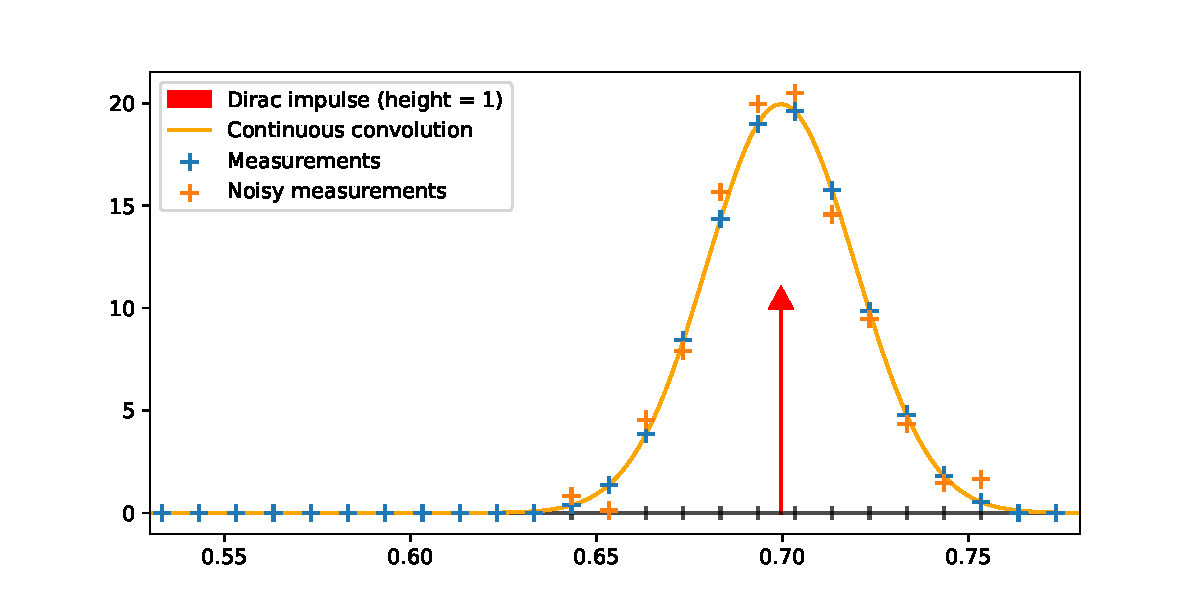
\includegraphics[width=\linewidth]{figures/simple_reco/measurement_figure.pdf}        
                \caption{Illustration of the effect of the measurement operator $\phib$ applied to a Dirac signal $\fb^\dagger = \delta_{x_0}$ with $x_0 \approx 0.695$.}
                \label{fig:simple:measop}
            \end{figure}

    
    \subsection{Composite representer theorem}

        As proposed, we address the deconvolution and signal separation task from \eqref{eq:ip-bis} using the two-variables optimization problem \eqref{eq:argminisback}. For a pair of parameters $\lambda_1, \lambda_2 > 0$ we consider

        \begin{equation}
        \label{eq:argmin-sps}
            \underset{(\fb,\fh) \in \mx \times \cHk}{\arg\min} \frac{1}{2} \| \bm{y} - (\phib (\fb) + \phih (\fh)) \|_2^2  + \lb \| \fb \|_{\mathcal{M}} + \frac{\lh}{2} \| \fh \|_{\cHk}^2.
        \end{equation}

        The solutions are indeed decoupled, according to the following result.
        \begin{proposition}
            \label{prop:rt-applied}
            Any solution to the optimization problem~\eqref{eq:argmin-sps} can be expressed as a pair of components $(s_1^*, s_2^*) \in \mx \times \cHk$ such that
            \begin{align}
                s_1^* &= \sum_{k=1}^{K_0} a_k \delta_{z_k}, \label{eq:deconv-banachpart}\\
                s_2^* &=  \frac{1}{\lh}\phih^* \mathbf{M}_{\lh}^{-1} \left(\bm{y} - \bm{w}\right),\label{eq:deconv-hilbertpart}
            \end{align}
            in which $(a_k, z_k)_k \in \left(\R \times \mathcal{X}\right)^{K_0} $ are amplitude-location pairs, $K_0 \leq L$, $\bm{w} = \phib(s_1^*)$ is independent on the actual solution $s_1^*$, and the matrix $\mathbf{M}_{\lambda_2} \in \R^{L \times L}$ is defined in equation \eqref{eq:def-Mphi}.
        \end{proposition}

        \begin{proof}
            By construction, Theorem~\ref{theo:main} holds for problem \eqref{eq:argmin-sps}. It directly leads to the expression of $s_2^*$ in $\eqref{eq:deconv-hilbertpart}$. Regarding the sparse component, we have that
            \begin{equation*}
                s_1^* \in \underset{ s_1\in\mx}{\arg\min} \quad  \mathcal{J}_{\mathbf{M}}(s_1)
            \end{equation*}
            with $\mathcal{J}_{\mathbf{M}}(s_1) := \|\mathbf{M}_{\lh}^{-\frac{1}{2}} ( \bm{y} - \phib(s_1)  ) \|_2^2  + \lb \| s_1 \|_{\mathcal{M}}$. From Proposition~\ref{prop:banachRT}, we know that this latter problem admits sparse solutions and that some can be expressed according to \eqref{eq:deconv-banachpart}.
        \end{proof}

        % \ju{Je mettrais le RT dans ce cas comme une proposition en étant clair sur le fait que c'est une application directe (à peine besoin d'une preuve)}
        % By construction, Theorem~\ref{theo:main} holds and the solution components are indeed decoupled.
        % With the matrix $\mathbf{M}_{\lambda_2} \in \R^{L \times L}$ defined in equation \eqref{eq:def-Mphi}, a solution of \eqref{eq:argmin-sps} is a pair of components $(s_1^\dagger, s_2^\dagger) \in \mx \times \ldx$ such that
        % \begin{align}
        %     s_1^* &\in \underset{ s_1\in\mx}{\arg\min} \quad  \mathcal{J}_{\mathbf{M}}(s_1), \label{eq:deconv-banachpart}\\
        %     s_2^* &=  \frac{1}{\lh}\phih^* \mathbf{M}_{\lh}^{-1} \left(\bm{y} - \bm{w}\right).\label{eq:deconv-hilbertpart}
        % \end{align}
        % with $\mathcal{J}_{\mathbf{M}}(s_1) = \|\mathbf{M}_{\lh}^{-\frac{1}{2}} ( \bm{y} - \phib(s_1)  ) \|_2^2  + \lb \| s_1 \|_{\mathcal{M}}$.
        % As stated in Theorem~\ref{theo:main}, $\bm{w} = \phib(s_1^*)$ does not depend on the recovered solution of \eqref{eq:deconv-banachpart}.
        % The smooth background problem \eqref{eq:deconv-hilbertpart} is explicit and only the sparse foreground estimation problem \eqref{eq:deconv-banachpart} needs to be solved numerically with optimization.
    
        % From Proposition~\ref{prop:banachRT}, we know that this latter problem admits sparse solutions and that some can be expressed as
        % \begin{equation*}
        %     s_1^* = \sum_k a_k \delta_{z_k}.
        % \end{equation*}
        
        The smooth background problem \eqref{eq:deconv-hilbertpart} is explicit, so that the only numerical challenge consists in estimating the positions $z_k \in \mathcal{X}$ and the associated intensities $a_k \in \R$ of the foreground component in \eqref{eq:deconv-banachpart}. The positions are notably more challenging to estimate than the intensities due to their continuously-defined nature and the nonlinear dependence on the measurements. This is done numerically by optimizing the single-component functional $\mathcal{J}_{\mathbf{M}}(\cdot)$ over $\mx$.
        The unique solution background component $s_2^*$ is then synthesized after computation of the residuals $\bm{y}-\bm{w}$ using \eqref{eq:deconv-hilbertpart}.

        \ad{
        \begin{remark}[Choice of the Hilbert space]
            The choice of the Hilbert space $\cH$ and in particular the Hilbert norm $\norm{\cdot}_\cH$ has a significant impact on the shape of $\fh^*$, involving the operator $\phih^*$ in equation~\eqref{eq:deconv-hilbertpart}. Classical choices consist in using the space of square integrable functions $\cH = \ldx$ equipped with the canonical norm $\norm{f}_{\ldx}^2 = \int_\cX f(x)^2 \mathrm{d}x$ for $f \in \ldx$, or alternatively introducing an invertible operator $\mathrm{L}_{\cH}: \ldx \to \ldx$ such that $\norm{f}_\cH^2 = \int_\cX \mathrm{L}_{\cH}\{f\}(x)^2 \mathrm{d}x $. However, these common norms generally do not permit to enforce a strong penalty on the high-frequency band of the solution, limiting their practical interest in applications.
            Our choice of using the RKHS induced by a Gaussian kernel is motivated by the test application considered in the following Section~\ref{sec:comp:reco}, in which we want to promote more energy in the low-frequency band. As demonstrated in equation~\ref{eq:rkhs-atom}, the reconstruction elements are shifted versions of the Gaussian function $g_t$ whose spatial extension is indeed larger than the measurement kernel $g$, hence promoting smoother solutions than what is achievable with classical $\mathrm{L}^2$-based norms.
        \end{remark}
        }
        
        % Finding a solution to \eqref{eq:deconv-banachpart} can then be reduced to the task of estimating some positions $z_k \in \mathcal{X}$ and the associated intensities $a_k \in \R$. The positions are notably more challenging to estimate than the intensities due to their their continuously-defined nature and the nonlinear dependence on the measurements.
        % The unique solution background component $s_2^*$ is then synthesized after computation of the residuals $\bm{y}-\bm{w}$ using \eqref{eq:deconv-hilbertpart}. 
        
    \subsection{Composite reconstruction}
    \label{sec:comp:reco}

        Some algorithms solve Problem \eqref{eq:argmin-sps}  directly on the continuum, such as the Sliding Frank-Wolfe \cite{denoyelle2019sliding} or the iterative refinement procedure of \cite{flinth2023grid}, however these methods can be long and computationally expensive to run.
        To put the emphasis on the decoupling of a composite solution, we decide here to simplify the solving by discretizing the foreground component estimation problem~\eqref{eq:deconv-banachpart}.
        
        % \ju{Question: ces méthodes peuvent résoudre un problem sparse comme (30) mais peuvent-elles résoudrent (29) en composite ?}\ad{Oui, si on utilise le RT de Debarre, qui permet de réduire la recherche de composante smooth en un problème de dimension finie. Dans ce cas, on peut calculer le gradient de (data fidelity + smooth regul) et appliquer les méthodes de types FW.}

    
        We do so by restricting the searched positions $z_k$ to live on a uniform fine grid. This approach alleviates the challenge of nonlinearity in the position parameters, turning \eqref{eq:deconv-banachpart} into a tractable finite dimensional generalized LASSO problem -- which can be large depending on the discretization interval and space dimensions. This strategy is usually adopted to approximate continuous-problem solutions \cite{simeoni2020functional,Debarre2019} and convergence toward gridless solutions has been studied (see \cite{duval2017sparseI,debarre2022part2} and the recent article \cite{guillemet2025a}). 
        % \ju{Tu peux ajouter le récent article de Vincent qui détaille cela plus loin que les autres résultats}

        We obtain the following finite-dimensional problem\footnotemark{} that approximates a continuous-domain solution of \eqref{eq:deconv-banachpart}:
        \begin{equation}
            \label{eq:gridbased-sparse}
            \underset{ \bm{a} \in \mathbb{R}^{J^d}}{\arg\min} \quad ( \bm{y} - \mathbf{H}\bm{a}  )^T \mathbf{M}_{\lh}^{-1} ( \bm{y} - \mathbf{H}\bm{a}  )  + \lb \| \bm{a} \|_{1},
        \end{equation}
        The $d$-dimensional grid contains $J^d$ knots and the vector $\bm{a}\in\R^{J^d}$ stores the amplitude of Dirac impulses located on the knots.
        The matrix $\mathbf{H} \in \R^{L \times J^d}$ accounts for the application of $\phib$ to grid-based Dirac impulses.
        In the simple case $d=1$, we obtain $\mathbf{H}[\ell, j] = g(x_{\ell} - z_j)$ for $1 \leq \ell \leq L $ and $1 \leq j \leq J$.
        \footnotetext{The discretization procedure is detailed in Appendix~\ref{app:discretization}.}
        
        The problem \eqref{eq:gridbased-sparse} can directly be solved with a proximal gradient descent algorithm (or any atomic LASSO solver such as a Frank-Wolfe algorithm). We solve this approximate problem considering a simple illustrative simulated example with $d=1$ in what follows.

        \subsubsection{Problem simulation and parametrization}

            We simulate a composite continuous-domain ground truth signal whose components are given by 
            $$s_1^{(0)} = \sum_{k=1}^{K_f} \beta_ k \delta(\cdot - u_k) \qquad\text{ and }\qquad s_2^{(0)} = \sum_{m=1}^{K_b} \gamma_m g_b(\cdot - v_m).
            $$
            The background component is built out of weighted replicas of the background Gaussian kernel $g_b = (1/\sqrt{2\pi\sigma_b^2}) \exp{(-x^2/(2 \sigma_b^2))}$ while the foreground involves sparse point sources. The locations $(u_k)_{k=1, \dots, K_f}$ and $(v_m)_{m=1, \dots, K_f}$ are drawn with a uniform distribution over the domain $[0, 1]$. The foreground is determined with $K_f = 10$ and $\beta_k$ drawn from a uniform distribution $\mathcal{U}([1, 10])$. The background parameters are $K_b = 100$ and $\gamma_m \sim \mathcal{U}([0.5, 1.5])$ with $\sigma_b = 0.08$.
            
            The measurement operator $\phib$ is defined with $L=100$ and $\sigma=0.02$. In addition, $\sigma_{\bm{n}}$ is set such that the signal-to-noise ratio between $\bm{y}$ and $\bm{n}$ reaches $SNR_\mathrm{dB} = 10 \log_{10}\left({\lVert \bm{y} \rVert_2^2}/{\lVert \bm{n} \rVert_2^2}\right) = 10$dB. To measure and adjust the contrast between the foreground and the background components in the signal to recover, we introduce the ratio $r_{1/2}$ of the contribution of each component in the observations, defined as
            \begin{equation}
                r_{1/2} = \frac{\lVert \phib (\fb^\dagger) \rVert_2 }{\lVert \phih (\fh^\dagger) \rVert_2 }.
            \end{equation}
    
            The observations $\bm{y}$ can be simulated with exact precision using this model. Indeed, we have
            $$
            \left[\phib(s_1^{(0)}) + \phih(s_2^{(0)})\right]_\ell = \sum_{k=1}^{K_f} \beta_k g(x_\ell - u_k) + \sum_{m=1}^{K_b} \gamma_m (g * g_b)(x_\ell - v_m),
            $$
            in which measuring the background involves the closed-form convolution
            $$
            (g\ *\ g_b)(x) = \frac{1}{\sqrt{2 \pi(\sigma^2 + \sigma_b^2)}} \exp{\left(-\frac{x^2}{2 (\sigma^2 + \sigma_b^2)}\right)}.
            $$
            
            We provide in figure~\ref{fig:simple:source} a simulated source signal built with a ratio of $r_{1/2} = 1$. 
            % \ju{après réflexion je me dis que tu peux garder la figure en expliquant bien l'effet d'échelle et le fait que la représentation peut être misleading.}
            The associated measurements are presented in figure~\ref{fig:simple:measurements}. Note that the contributions of the two components $\phib(\fb^\dagger)$ and $\phih(\fh^\dagger)$ have the same Euclidian norm although their distribution of mass is very different, leading to the misleading difference of scales in the right panel of figure~\ref{fig:simple:measurements}. %In this case, the $\ell_1$-norm of the contribution of the background is actually twice as large as the one from the foreground.
    
            \begin{figure}[t]
                \centering
                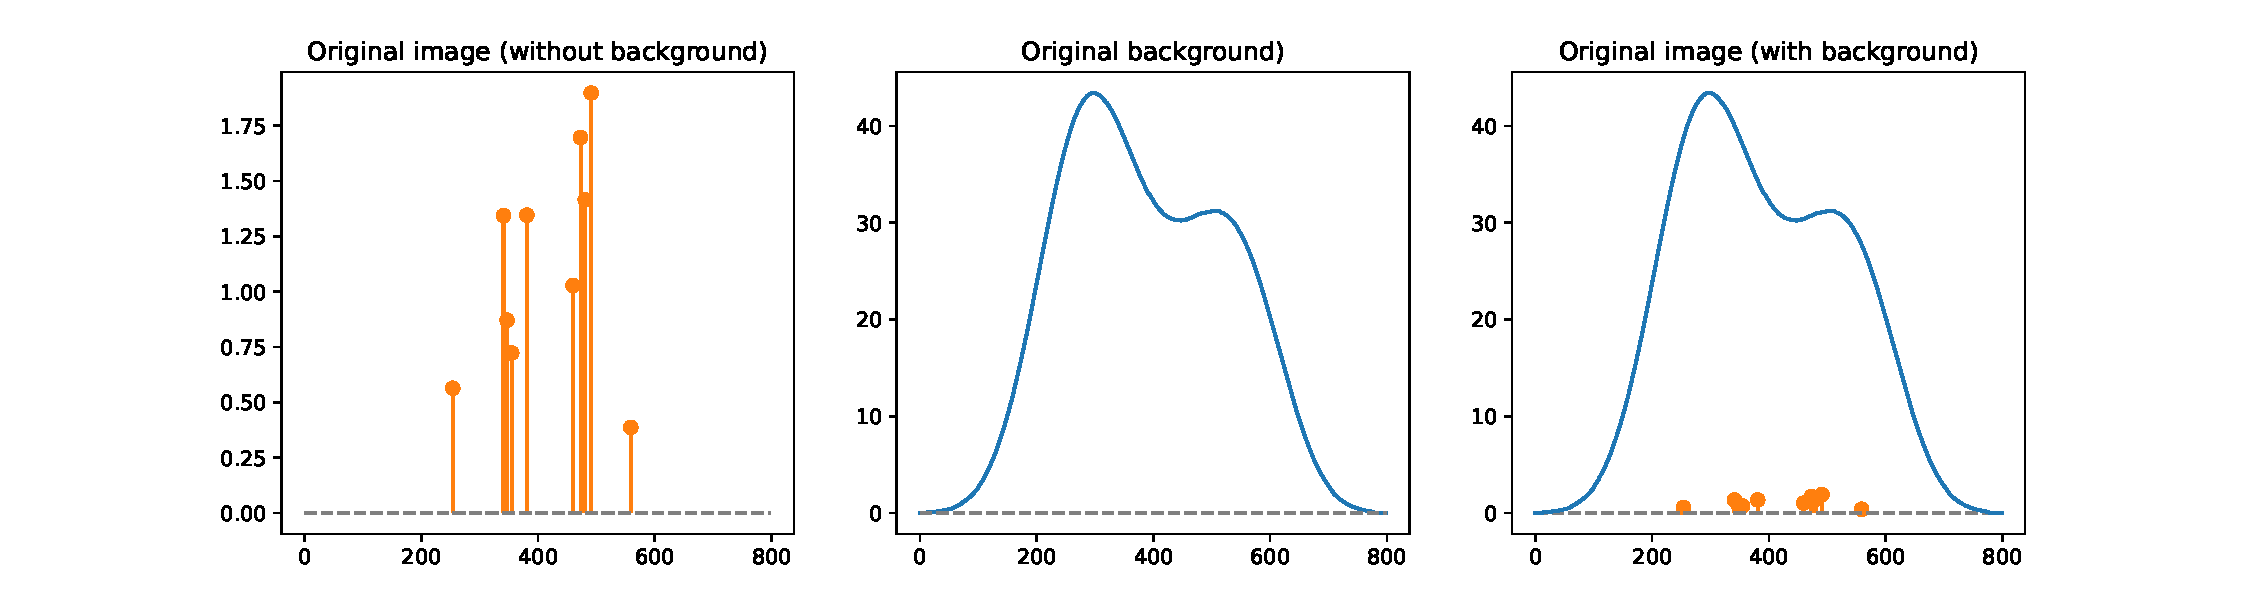
\includegraphics[width=\linewidth]{figures/simple_reco/gt.pdf}        
                \caption{Simulated source signal. \textit{Left:} Sparse component. \textit{Center:} Background smooth component. \textit{Right:} Sum of the two components.}
                \label{fig:simple:source}
            \end{figure}
        
            \begin{figure}[t]
                \centering
                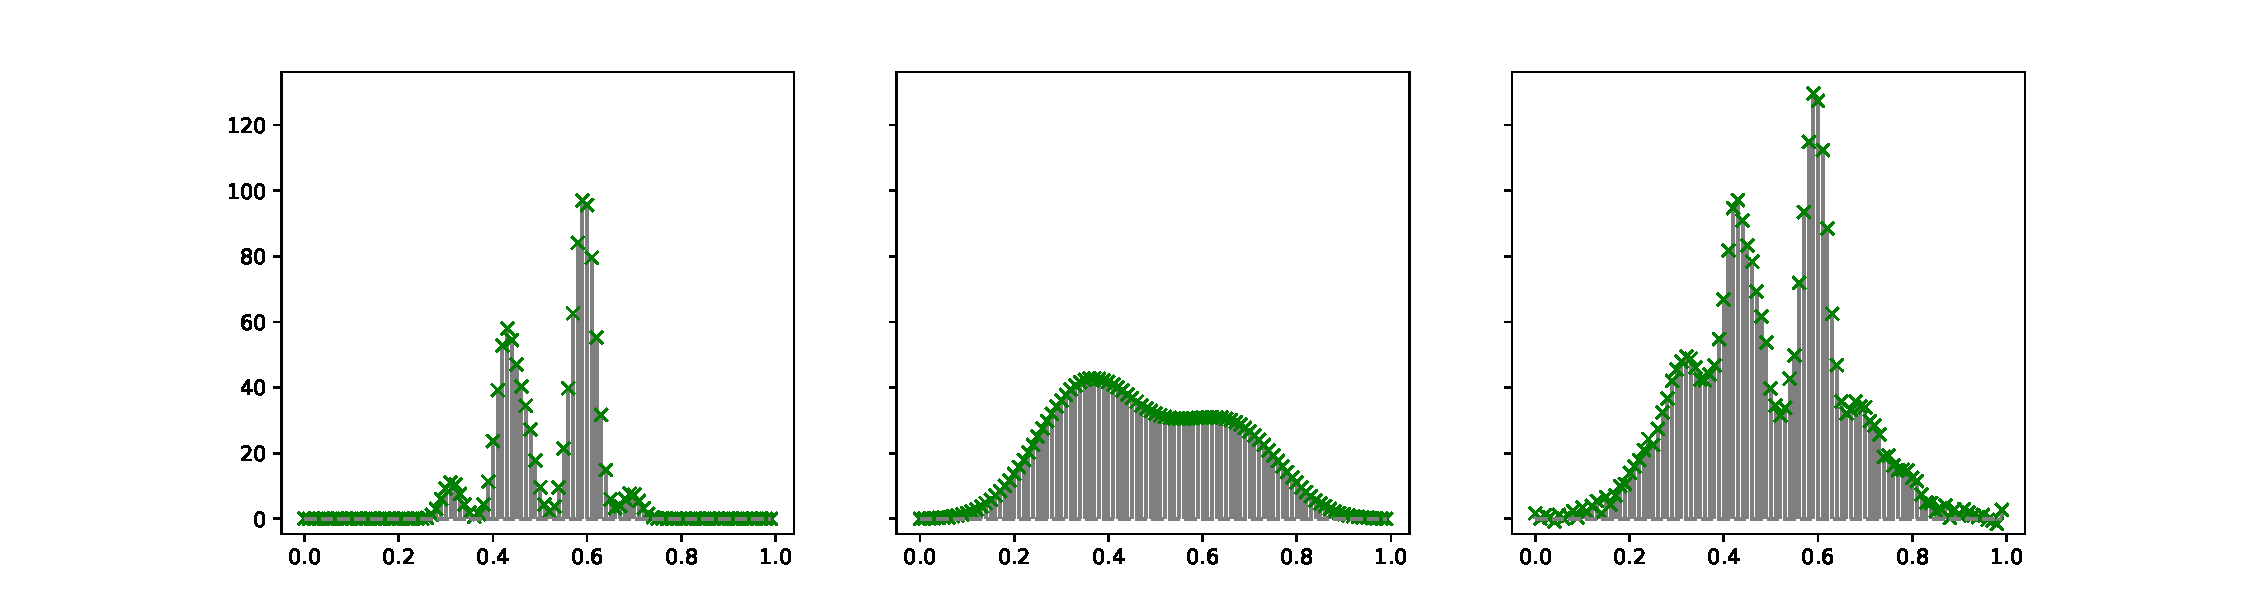
\includegraphics[width=\linewidth]{figures/simple_reco/measurements.pdf}        
                \caption{Simulated measurements. \textit{Left:} Contribution of the sparse component. \textit{Center:} Contribution of background. \textit{Right:} Total noisy observations $\bm{y}$. In practice, only the information of the right-hand plot are accessible and the problem does not know the respective contribution of the components.}
                \label{fig:simple:measurements}
            \end{figure}

        \subsubsection{Reconstruction of the signals}
        For a fine resolution reconstruction, the grid size is set to $J = n_\mathrm{srf} . L$ with the super-resolution factor fixed to $n_\mathrm{srf}=8$. The penalty parameters are tuned manually based on scaling rules to maintain values in a range consistent with the inverse problem. We set $\lh = \alpha_2 L$ with a real-valued coefficient $\alpha_2 >0$ (see Appendix~\ref{app:calculation} for a justification).
        %According to equation~\eqref{eq:def-Mphi}, the parameters $\lh$ appears in the sparse component estimation problem in front of the Gram matrix as $(1/\lh)\phih\phih^*$. It is then relevant to scale $\lh$ with the highest singular value of $\phih$, which is $\sigma_{mas}(\phih)\approx L$ in our case.
        Once $\lh$ has been set, $\lb$ is fixed as a rate of the maximum value as defined in \eqref{eq:l1max} with $\lb = \alpha_1 \lambda_{1, \mathrm{max}}$ for $0 < \alpha_1 <1$. Typically, $\alpha_1$ takes values in the range $[0.1, 0.3]$. To emphasize the smoothing effect on the background, we use the reconstruction width $\sigma_t = 0.1 > \sigma_b$.

        Figure~\ref{fig:simple:recos} presents the foreground and background components recovered with regularization parameters $\lambda_2 = 0.08 L =8$ and $\alpha_1 = 0.25$. Additionally, a positivity constraint has been enforced on $s_1$ which does not break the representer theorem and usually improves the quality of the reconstruction. We used an APGD algorithm \cite{liang2022improving} to solve the approximate decoupled problem \eqref{eq:gridbased-sparse}.

        \begin{figure}[t]
            \centering
            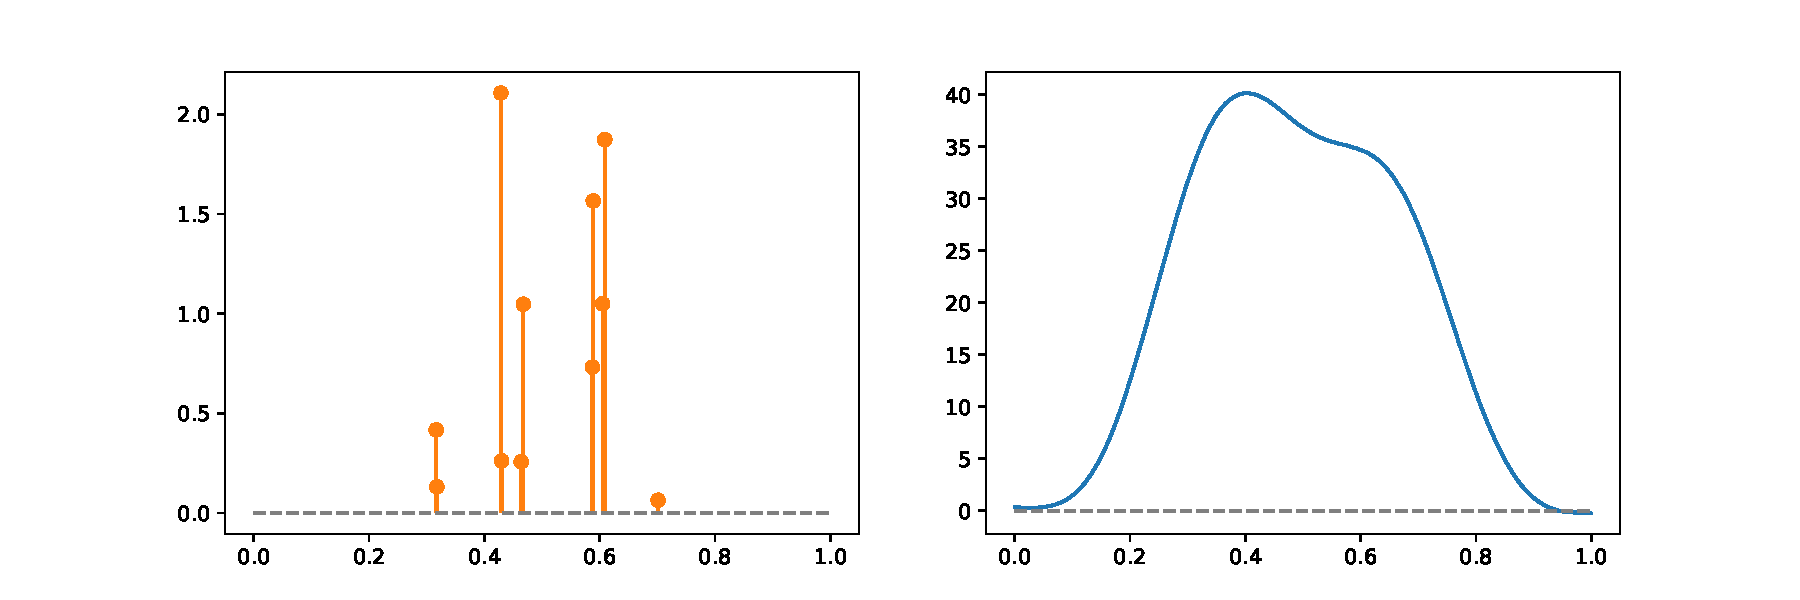
\includegraphics[width=\linewidth]{figures/simple_reco/recos.pdf}        
            \caption{Recovered signals with regularization parameters $\lambda_2 = 10^{-2}$ and $\alpha = 0.2$. \textit{Left:} Sparse foreground component. \textit{Right:} Smooth background.}
            \label{fig:simple:recos}
        \end{figure}

        The sparse component is similar to the simulated source signal of figure~\ref{fig:simple:source} although many reconstructed peaks are composed of several small intensity impulses, which makes the comparison with the ground truth difficult. The background component is less faithful. The overall intensity matches the intensity of the ground truth but the local variations are not correctly captured, we observe for instance high intensity around the coordinate $0.7$ which could correspond to a leakage from the foreground component. Additionally, we  observe a plateau effect in the recovered background information, reaching here the value $35$. This plateau is systematic in the reconstructions (as can be seen in Appendix~\ref{app:reconstructions}) and could be due to the LASSO problem, which outputs a residual of bounded intensity.

        This difficulty to accurately recover the background may not be critical in practice as one is usually interested in accurate reconstruction of the foreground component. To provide a better comparison between the source foreground component and the recovered one, we convolve the sparse signals $s_1^*$ and $s_1^\dagger$ with a representation kernel. We use a narrow Gaussian function of small standard deviation $\sigma_r = \sigma/4$. This operation intuitively blends nearby peaks while respecting the spatial spread of different clusters. The resulting signals are displayed in figure~\ref{fig:simple:recos-conv}, demonstrating consistency between the signals.
        % \ad{Should I comment more ?}
        % The $K_f=10$ source peaks are recovered. Some of them suffer from a small intensity shrinkage, which is a well-known artefact of LASSO-like problems. Spurious peaks are also reproduced around the left peak, which may be explained by the presence of strong background information around this location. 
        
        \begin{figure}[t]
            \centering
            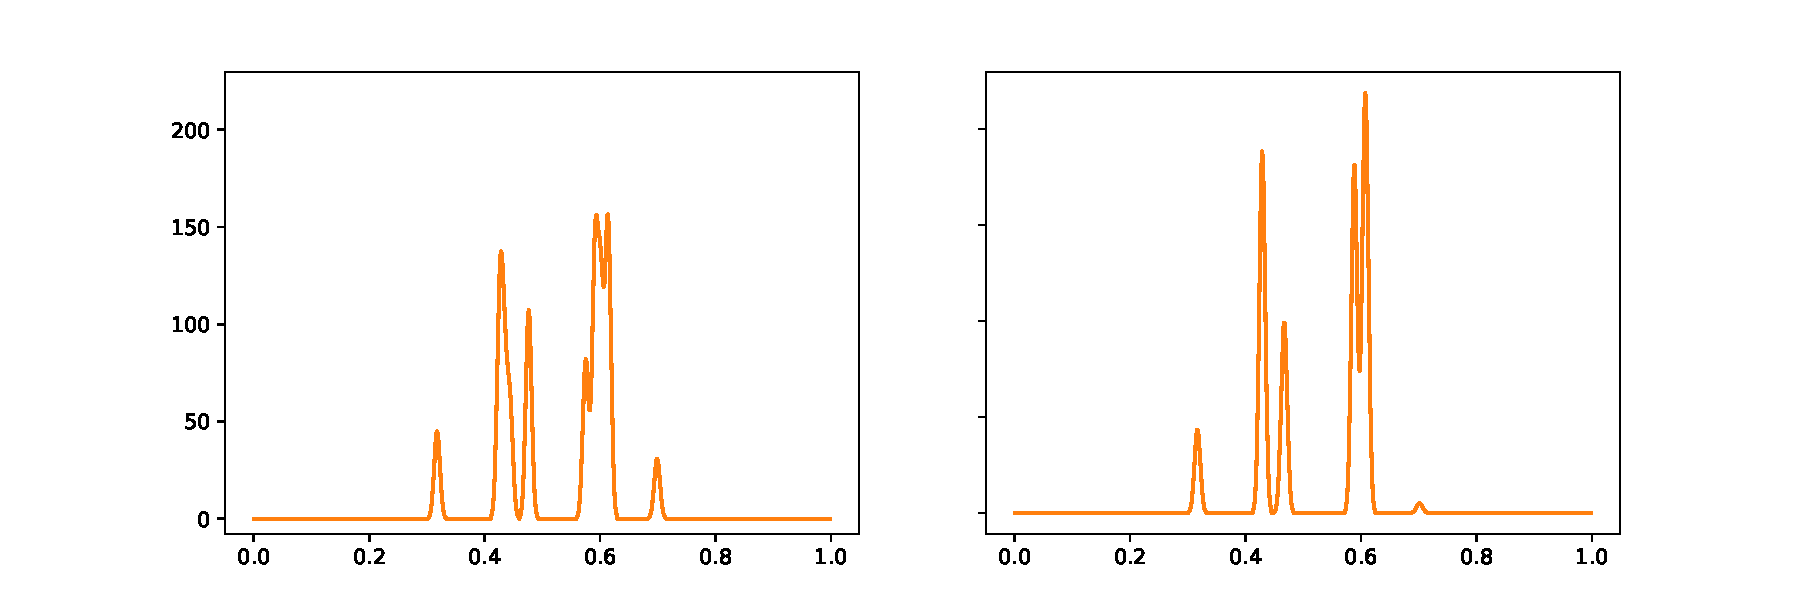
\includegraphics[width=\linewidth]{figures/simple_reco/recos_conv.pdf}        
            \caption{Foregrounds convolved with the sharp representation kernel. \textit{Left:} Ground truth signal. \textit{Right:} Reconstruction.}
            \label{fig:simple:recos-conv}
        \end{figure}

        Obviously, the penalty parameters $\lb$ and $\lh$ have a significant influence on the recovered components and the interplay between the respective value of these two parameters is not fully understood. We provide in Appendix~\ref{app:reconstructions} a cross table of reconstructions with various regularization parameters to illustrate the dependence. 
        
\section{Benefits of our Decoupled Composite Model}
    
    Building on the simulated composite model presented in the previous section, we now illustrate the benefits of our approach.
    
    First, composite modeling accurately recovers the unknown signal in situations where single-component problems fail to distinguish foreground from background information. Second, using a decoupled numerical procedure reduces the computation time compared to a direct 2-variables approach of the composite optimization problem.

    The numerical experiments in this section have been implemented with the Python programming language based on the optimization package \texttt{Pyxu} \cite{pyxu-framework}. All the simulations have run on a workstation with 2 CPUs Intel Xeon E5-2680 v3 \@2.5 Ghz, 30 MB cache and 24 threads each. 

    \subsection{Compared to single-component model}
    \label{sec:bene:comp}
        In applications where only the foreground component is of interest, we may wonder if using a composite model is relevant in the first place. Would it be possible to simply recover the foreground with a single-component sparsity-promoting problem only? We address the question in this section, first visually then introducing evaluation metrics.

        \subsubsection{Single-component reconstruction}
        Using the same composite ground truth signal $(s_1^\dagger, s_2^\dagger)$ as in Section~\ref{sec:comp:reco}, we consider the following single-component B-LASSO problem with still the same measurement operator $\phih$ and the same observations $\bm{y}\in\R^L$:
        \begin{equation}
            \label{eq:argmin-sparse-only}
            \underset{\fb \in \mx}{\arg\min} \frac{1}{2} \| \bm{y} - \phib (\fb) \|_2^2  + \lambda \| \fb \|_{\mathcal{M}},
        \end{equation}
        for $\lambda > 0$.
        With the fine-grid discretization proposed above, finding an approximate grid-based solution of this problem amounts to solve a classical LASSO problem. The regularization parameter $\lambda > 0$ is set specifically for this problem and is independent of $\lb$ used in \eqref{eq:deconv-banachpart}. There also exists a maximum value $\lambda_\mathrm{max} = \norm{\phib^*\bm{y}}_\infty$ for problem~\eqref{eq:argmin-sparse-only} and we set $\lambda = \alpha \lambda_\mathrm{max}$ for $0 < \alpha < 1$. It is usually larger than $\lambda_1$ as we need stronger prior information to recover a sparse solution.
        
        Figure~\ref{fig:simple:blasso-conv} displays the reconstructions with the same representation kernel as before for various reconstruction parameters $\alpha$.
        We observe that the B-LASSO problem manages to recover some high intensity peaks, however the reconstructions are strongly corrupted by the presence of background information. When more sparsity is enforced with a larger value of $\alpha$, the spurious peaks tend to vanish but the intensity of the relevant peaks is also reduced, becoming lower than the source and than the composite reconstruction.

        \begin{figure}[t]
            \centering
            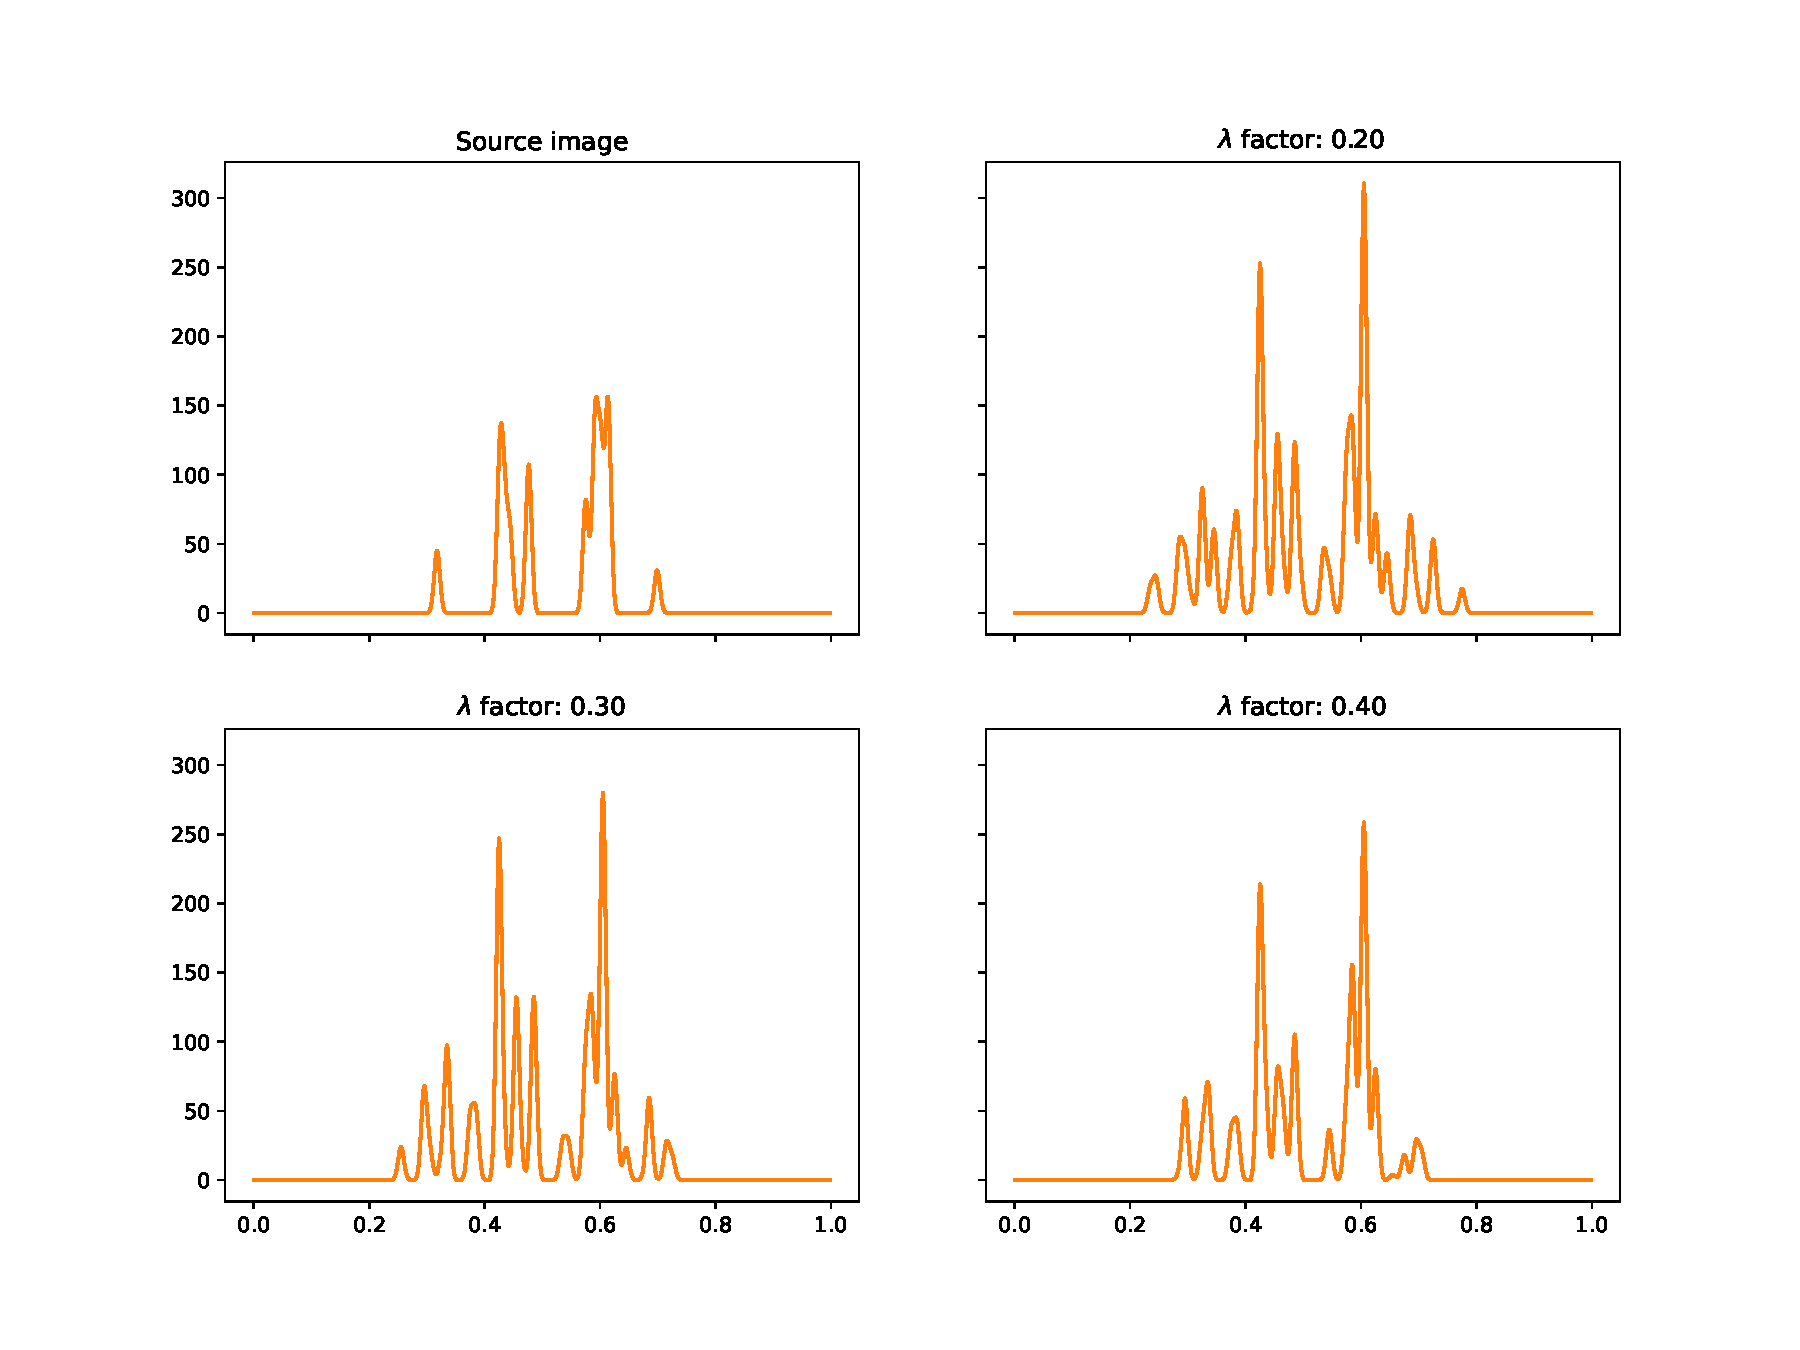
\includegraphics[width=\linewidth, trim=0 2cm 0 2.2cm, clip]{figures/simple_reco/blasso_merged.pdf}
            \caption{Single-component reconstructions using a B-LASSO problem approximated on the fine grid: ground truth (\textit{upper left}) and several values of the regularization parameter ($\alpha=0.2, 0.3$ or $0.4$). \ad{Larger titles or subfigures.}}
            \label{fig:simple:blasso-conv}
        \end{figure}
        
        \subsubsection{Quantitative study}

        Assessing the quality of the reconstruction of sparse signal is always a complicated task as both intensity and localization of the recovered sources need to be simultaneously evaluated. We consider two simple metrics based on the grid-based representation of the recovered foreground. First, the ground truth and the solution are convolved with the representation Gaussian kernel. Second, the relative error is computed using either $\mathrm{L}^2$-norm or the $\mathrm{L}^1$-norm. For $\fb$ the recovered foreground component, $\fb^\dagger$ the simulated source and $g_{\sigma_r}$ the representation kernel, we define
        $$
        \mathrm{RE}_2(\fb, \fb^\dagger) = \frac{\lVert g_{\sigma_r} * (\fb - \fb^\dagger) \rVert_2 }{ \lVert g_{\sigma_r} * \fb^\dagger \rVert_2} \qquad\text{and}\qquad
        \mathrm{RE}_1(\fb, \fb^\dagger) = \frac{\lVert g_{\sigma_r} * (\fb - \fb^\dagger) \rVert_1}{\lVert g_{\sigma_r} *\fb^\dagger \rVert_1}.
        $$
        The metrics are approximated using the fine-grid representation of the signals.

        The evaluation metrics on the foreground component are reported in tables~\ref{tab:rl2} and~\ref{tab:rl1} for the sparse-plus-smooth composite model, and in table~\ref{tab:blasso} for the single-component reconstructions with the B-LASSO. The parameters chosen for figures~\ref{fig:simple:recos} and~\ref{fig:simple:recos-conv} correspond to the best pair $\lambda_2 = 0.08 L$ and $\alpha_1=0.25$, the reconstructions obtained with the other parameters are displayed in Appendix~\ref{app:reconstructions}.

        % The best B-LASSO reconstruction is consistently outperformed by most of the composite reconstructions. \ju{Comme dit ailleurs, je ne comprends pas pourquoi les expériences te permettent de dire ça vu que tu considère deux problèmes différents. Pourquoi ne pas prendre $s$ au lieu de $s_1$ qui montrerait que le Lasso a visuellement et quantitativement mieux ? To be discussed.}
        The two metrics produce consistent results as they both identify the same best solution, although the values and the gaps between the methods are different. The metrics for the B-LASSO improve with higher values of the penalty parameter, coincidentally with a decrease in intensity of the recovered signal. This observation may suggest that the B-LASSO model is inappropriate for such a recovery problem and having a composite model improves the reconstruction. 
        
        \begin{table}[b]
        \centering
        \begin{subtable}[t]{0.45\linewidth}
            \centering
            \begin{tabular}{l|rrrr}
                \toprule
                 & \multicolumn{4}{c}{$\alpha_2$ in $\lambda_2 = \alpha_2 L$} \\
                \cmidrule(lr){2-5}
                $\alpha_1$ & 0.80 & 4.00 & 8.00 & 40.00 \\
                \midrule
                0.02 & 0.503 & 0.728 & 0.798 & 1.047 \\
                0.05 & 0.567 & 0.592 & \textbf{0.440} & 1.075 \\
                0.10 & 0.637 & 0.595 & 0.571 & 0.839 \\
                0.15 & 0.826 & 0.805 & 0.647 & 0.516 \\
                \bottomrule
            \end{tabular}
            \caption{Relative $\ell_2$-norm error \label{tab:rl2}}
        \end{subtable}
        \hfill
        \begin{subtable}[t]{0.45\linewidth}
            \centering
            \begin{tabular}{l|rrrr}
                \toprule
                 & \multicolumn{4}{c}{$\alpha_2$ in $\lambda_2 = \alpha_2 L$} \\
                \cmidrule(lr){2-5}
                $\alpha_1$ & 0.80 & 4.00 & 8.00 & 40.00 \\
                \midrule
                0.02 & 0.495 & 1.070 & 1.297 & 1.748 \\
                0.05 & 0.585 & 0.601 & 0.626 & 1.669 \\
                0.10 & 0.647 & 0.593 & \textbf{0.571} & 1.196 \\
                0.15 & 0.802 & 0.790 & 0.661 & 0.600 \\
                \bottomrule
            \end{tabular}
            \caption{Relative $\ell_1$-norm error\label{tab:rl1}}
        \end{subtable}
        \caption{Evaluation metrics for the composite reconstructions.}
        \end{table}
    
        \begin{table}[b]
            \centering
            \begin{tabular}{l|rrrr}
                \toprule
                 & \multicolumn{4}{c}{$\alpha$ in $\lambda = \alpha \lambda_{\mathrm{max}}$} \\
                \cmidrule(lr){2-5}
                 & 0.10 & 0.20 & 0.30 & 0.40 \\
                \midrule
                $\mathrm{RE}_2$ & 1.126 & 1.033 & 0.953 & \textbf{0.783} \\
                $\mathrm{RE}_1$ & 1.864 & 1.593 & 1.370 & \textbf{1.051} \\
                \bottomrule
            \end{tabular}
            \caption{B-LASSO errors \label{tab:blasso}}
        \end{table}

        To further compare the interest of using a composite model over a single-component one, we study how the reconstruction metrics evolve with respect to the contrast of the signal to recover, that is the relative importance between the foreground and background components. We run the same experiment while varying the parameter $r_{1/2}$ and we report in figure~\ref{fig:bench:metrics-vs-r} the best value of the metric obtained through various sets of regularization parameters.

        Independently of the contrast and the metric used, the composite model systematically outperforms the single-component one. With higher values of contrast, that is when the foreground gets more intense relative to the background, both model reduce their error metrics and thus produce better reconstructions. Interestingly, the gap between the methods also shrinks with the contrast, ultimately being almost nonexistent for $r_{1/2} = 4$. It suggests that for sufficiently high contrasts, sparse single-component modeling may be enough to obtain an accurate reconstruction of the foreground.

        \begin{figure}[t]
            \centering
            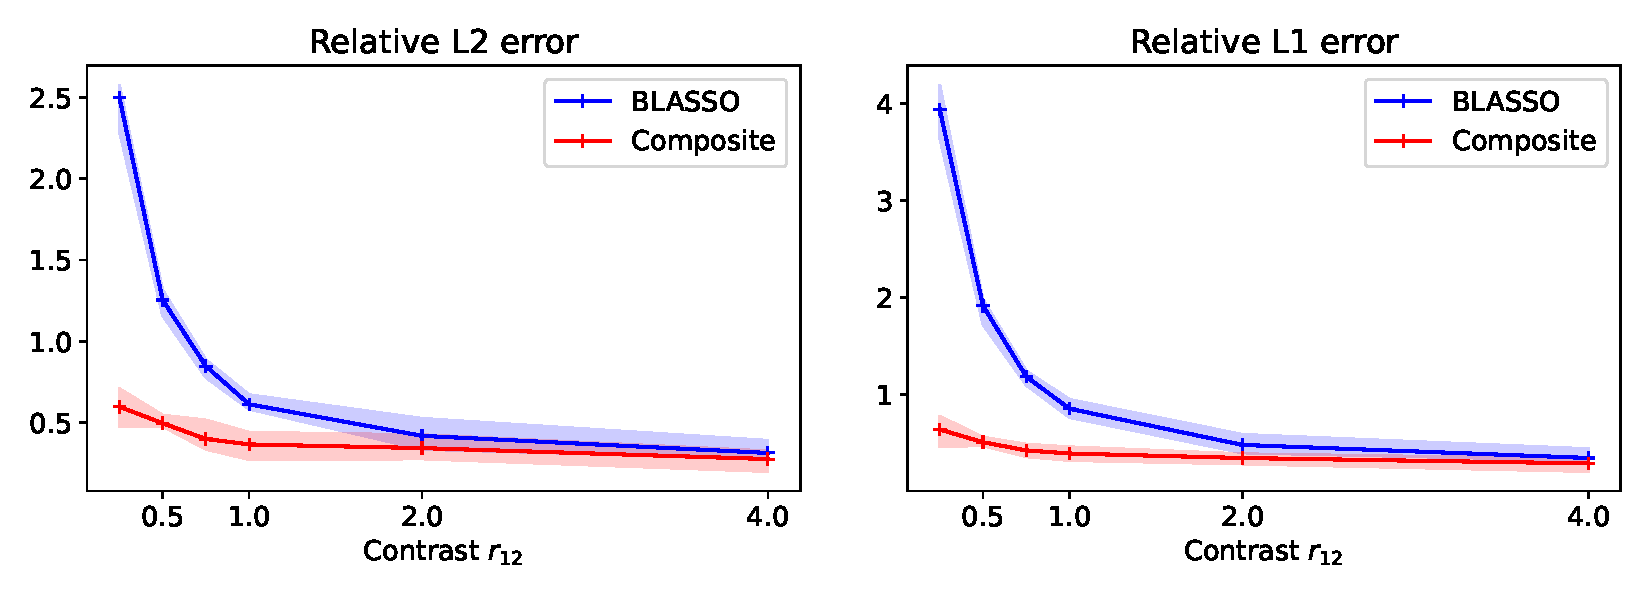
\includegraphics[width=\linewidth]{figures/benchmark/error_vs_r12.pdf}        
            \caption{Relative error with respect to contrast. For each value of $r_{1/2}$, 24 problems are simulated and solved, the median values and interquartile spreads are respectively shown with solid line and shaded area. \textit{Left:} Using $RE_2$. \textit{Right:} Using $RE_1$.}
            \label{fig:bench:metrics-vs-r}
        \end{figure}


    \subsection{Compared to a non-decoupled solver}
    \label{sec:bene:deco}
        So far we have illustrated Theorem~\ref{theo:main} and highlighted the interest of using a composite model in the presence of a smooth background signal. The main contribution of our theorem consists in the decoupling of the composite optimization problem and its practical benefits unveil when comparing the solving time with a direct non-decoupled approach. 

        \subsubsection{Non-decoupled approach}
        Letting apart Theorem~\ref{theo:main}, the composite optimization \eqref{eq:argmin-sps} can also be treated directly using the representer theorem of \cite{debarre2021continuous}. Indeed, it was known that there exists at least one Dirac-based sparse solution for the foreground component as
        \begin{equation}
            s_1^* = \sum_{k=1}^{K_1} a_{k} \delta(\cdot - x_k)
            \label{eq:rt-deb-1}
        \end{equation}
        with $a_{k} \in \mathbb{R}$, $x_k \in \mathcal{X}$ and $K_1 \leq L$.
        Additionally, the background component was known to be unique and that it can be expressed as
        \begin{equation}
            s_2^* = \sum_{\ell=1}^{L} b_{\ell} \phi_\ell,
            \label{eq:rt-deb-2}
        \end{equation}
        with $b_\ell \in \mathbb{R}$ and $\phi_\ell$ the measurement functionals.

        Plugging \eqref{eq:rt-deb-1} after discretization on the fine grid $G_J$ and \eqref{eq:rt-deb-2} into the composite minimization cost function \eqref{eq:argmin-sps}, we obtain the following two-components optimization problem of dimension $J^d + L$, that we refer to as the \emph{non-decoupled approach} :
        \begin{equation}
        \label{eq:ndcp-argmin}
            \underset{(\mathbf{a}, \mathbf{b})\ \in\ \R^{J^d} \times \R^L}{\arg\min} \frac{1}{2} \| \bm{y} - \mathbf{Ha} - \mathbf{Tb} \|_2^2  + \lb \| \mathbf{a} \|_1 + \frac{\lh}{2} \langle \mathbf{b}, \mathbf{Tb} \rangle,
        \end{equation}
        where the matrix $\mathbf{T} \in \R^{L \times L}$ is defined as
        % $\mathbf{T}[i, j] = \langle \phi_j, \phi_i\rangle$ for $1 \leq i, j \leq L$
        $\mathbf{T}[i, j] = (g * g_0 * g)(x_j - x_i)$ for $1 \leq i, j \leq L$
        and $\mathbf{H} \in \R^{L\times J^d}$ is from \eqref{eq:gridbased-sparse}.
        % \ju{do you specify what is $T$ and how it connects with our theorem? + recall what is $H$ maybe.}
        This problem is equivalent to our decoupled and discretized approach \eqref{eq:deconv-banachpart} and \eqref{eq:deconv-hilbertpart}. It is convex, finite-dimensional, and the terms are either differentiable or proximable so that the optimization can be performed with a proximal algorithm. In what follows, we solve it with APGD. % and refer to this approach as \emph{non-decoupled}.
    
        \subsubsection{Quantitative assessment}
        As mentioned with Proposition~\ref{prop:rt-applied}, the composite optimization problem \eqref{eq:argmin-sps} can be solved by performing an optimization procedure on the foreground component only.
        %The numerical procedure get simplified as only one variable needs to be considered.
        To asses the practical benefits of such transformation, we compare the runtime of the decoupled solver, including the a posteriori computation of the background component, with the non-decoupled approach of solving the two-components problem~\eqref{eq:ndcp-argmin}. For completeness, we also include in our comparison the runtime for solving a B-LASSO problem with the same input.

        For a fair treatment between the solver, the stopping criterion of all the algorithms is set as a threshold on the relative improvement of consecutive iterates of the foreground component variable. We present two experiment: the first one, displayed in figure~\ref{fig:time-vs-r}, reports the reconstruction time when the contrast $r_{1/2}$ evolves in the same setup as in section~\ref{sec:bene:comp}; the second experiment is reported in figure~\ref{fig:time-vs-srf} and presents the reconstruction time when the super resolution factor $n_\mathrm{srf}$ varies. The times reported correspond to the best reconstruction obtained through a tested set of regularization parameters. Each experiment is reproduced 24 times, the median value is reported with the solid line and the shaded area represents the interquartile spread.
        % \ju{I don't see where NDCP is presented, commented and linked with some previous works. I am right?}

        \begin{figure}[t]
            \centering
            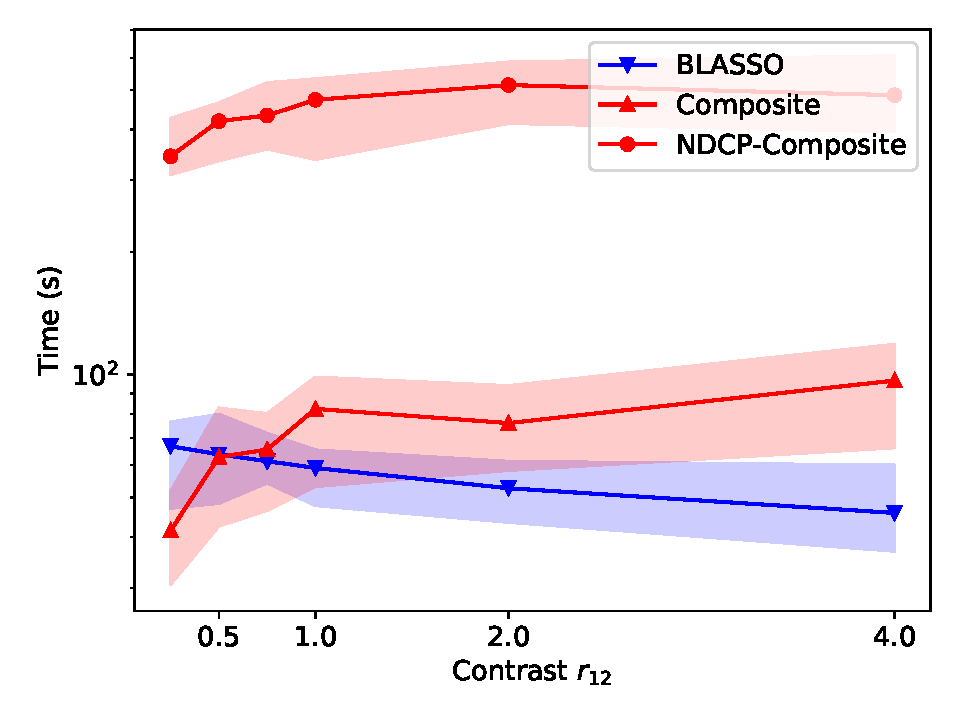
\includegraphics[width=.7\linewidth]{figures/benchmark/time_vs_r12.pdf}        
            \caption{Time for the best reconstruction with the different solvers with varying values of $r_{1/2}$ and fixed value of $n_\mathrm{srf} = 8$. The two composite approaches are in red, with triangle markers for the decoupled reconstruction and circle for the non-decoupled problem (``NDCP'' in the legend).}
            % \ju{I wonder what happens with a log scale. We shall see more easily the gain with the BLASSO.}
            \label{fig:time-vs-r}
        \end{figure}
    
        \begin{figure}[t]
            \centering
            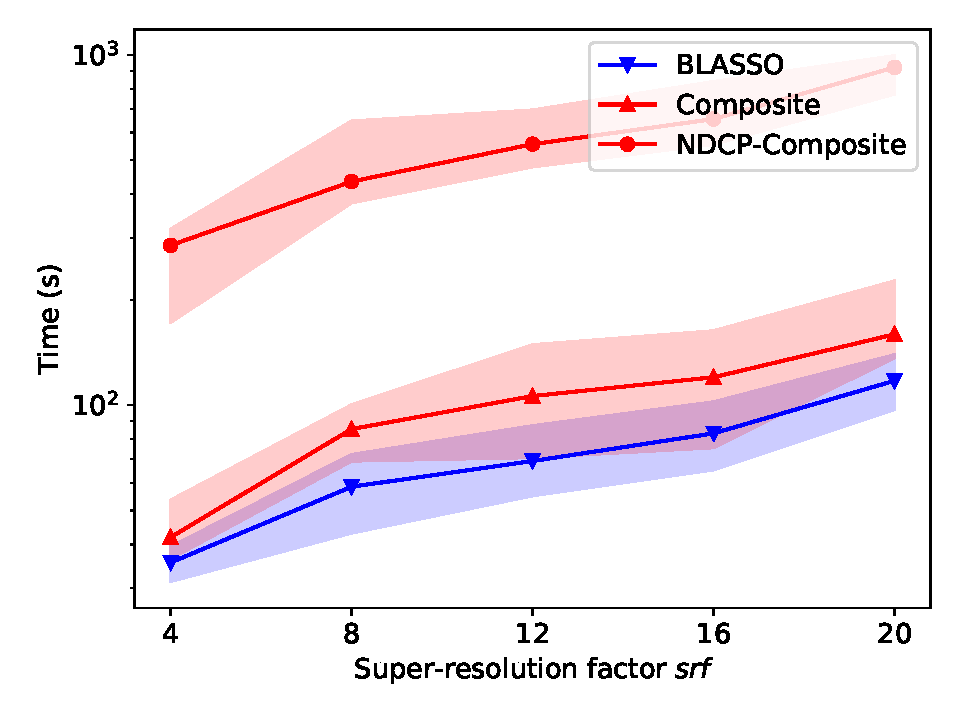
\includegraphics[width=.7\linewidth]{figures/benchmark/time_vs_srf.pdf}        
            \caption{Time for the best reconstruction with the different solvers with varying values of $n_\mathrm{srf}$ and fixed $r_{1/2}=1$.}
            \label{fig:time-vs-srf}
        \end{figure}
    
        \ad{Update the figures.}
        On both scenarios, the decoupled approach run significantly faster than the non-decoupled one, on average taking 10.6\% of the runtime in the first experiment (varying contrast) and 8.9\% in the second one (varying super resolution factor). Up to numerical approximations, the solutions are identical between the two methods. Interestingly, the decoupled approach turns out to be faster than the regular B-LASSO solver. Varying the contrast $r_{1/2}$ has little effect on the reconstruction time. Increasing the resolution, that is using more grid points in the discrete representation of $s_1^*$, slows down the solving for all the algorithms. The effect is stronger for the non-decoupled method, which suffers from having its reconstruction time multiplied by approximately $3.5$.

        